\chapter{Aquisição e Tratamento dos Dados}
\date{24}{03}{2015}
\section{Aquisição de Dados}

No âmbito do projeto SUBSAL, realizado conjuntamente entre o Observatório Nacional e a Petrobras,  instalou-se 24 estações sismográficas temporárias banda larga (STS2 ou Reftek RT151-120s), as coordenadas de cada estação podem ser vistas na Tabela \ref{tabelaDATA}. A faixa de frequência registrada varia de 50 Hz até 100 segundos. Acoplado a este sistema temos um conjunto de baterias, reguladores, painel solar e o registrador, onde são armazenados os dados. O sistema armazena os dados em um disco de 4Gb que é retirado em cada campanha de coleta dos dados.

Mesmo se tratando de estações temporárias, as instalações devem conter os requisitos mínimos para a uma aquisição confiável dos dados. Principalmente assegurar que o sensor e o registrador não sofram com as intempéries climáticas ou com danos causados pela passagem de animais ou pessoas pelo local. A Figura \ref{instalacao} mostra como é o fluxo de trabalho dos funcionários do Observatório Nacional no campo para a instalação das estações sismográficas temporárias. 

A Figura \ref{instalacao}-A mostra que o sensor deve ser acoplado à rocha sã. Com a ajuda de uma bússola, o sensor é orientado segundo um azimute.  Porém para um isolamento térmico, crucial para o bom funcionamento do sismômetro, pinta-se a área com um tinta isolante e o sismômetro é revestido com uma manta térmica, como pode ser visto na A Figura \ref{instalacao}-B e \ref{instalacao}-C. Logo após instala-se as baterias e o sensor é mais uma vez revestido. Para a absorçao da umidade de todo o sistema da estaçao, utiliza-se carvão e sílica em gel, como pode ser visto na Figura \ref{instalacao}-D. Em seguida todo o sistema é coberto e cercado como pode ser visto nas Figuras \ref{instalacao}-E e \ref{instalacao}-F.	  

\begin{figure}[!ht]
\centering
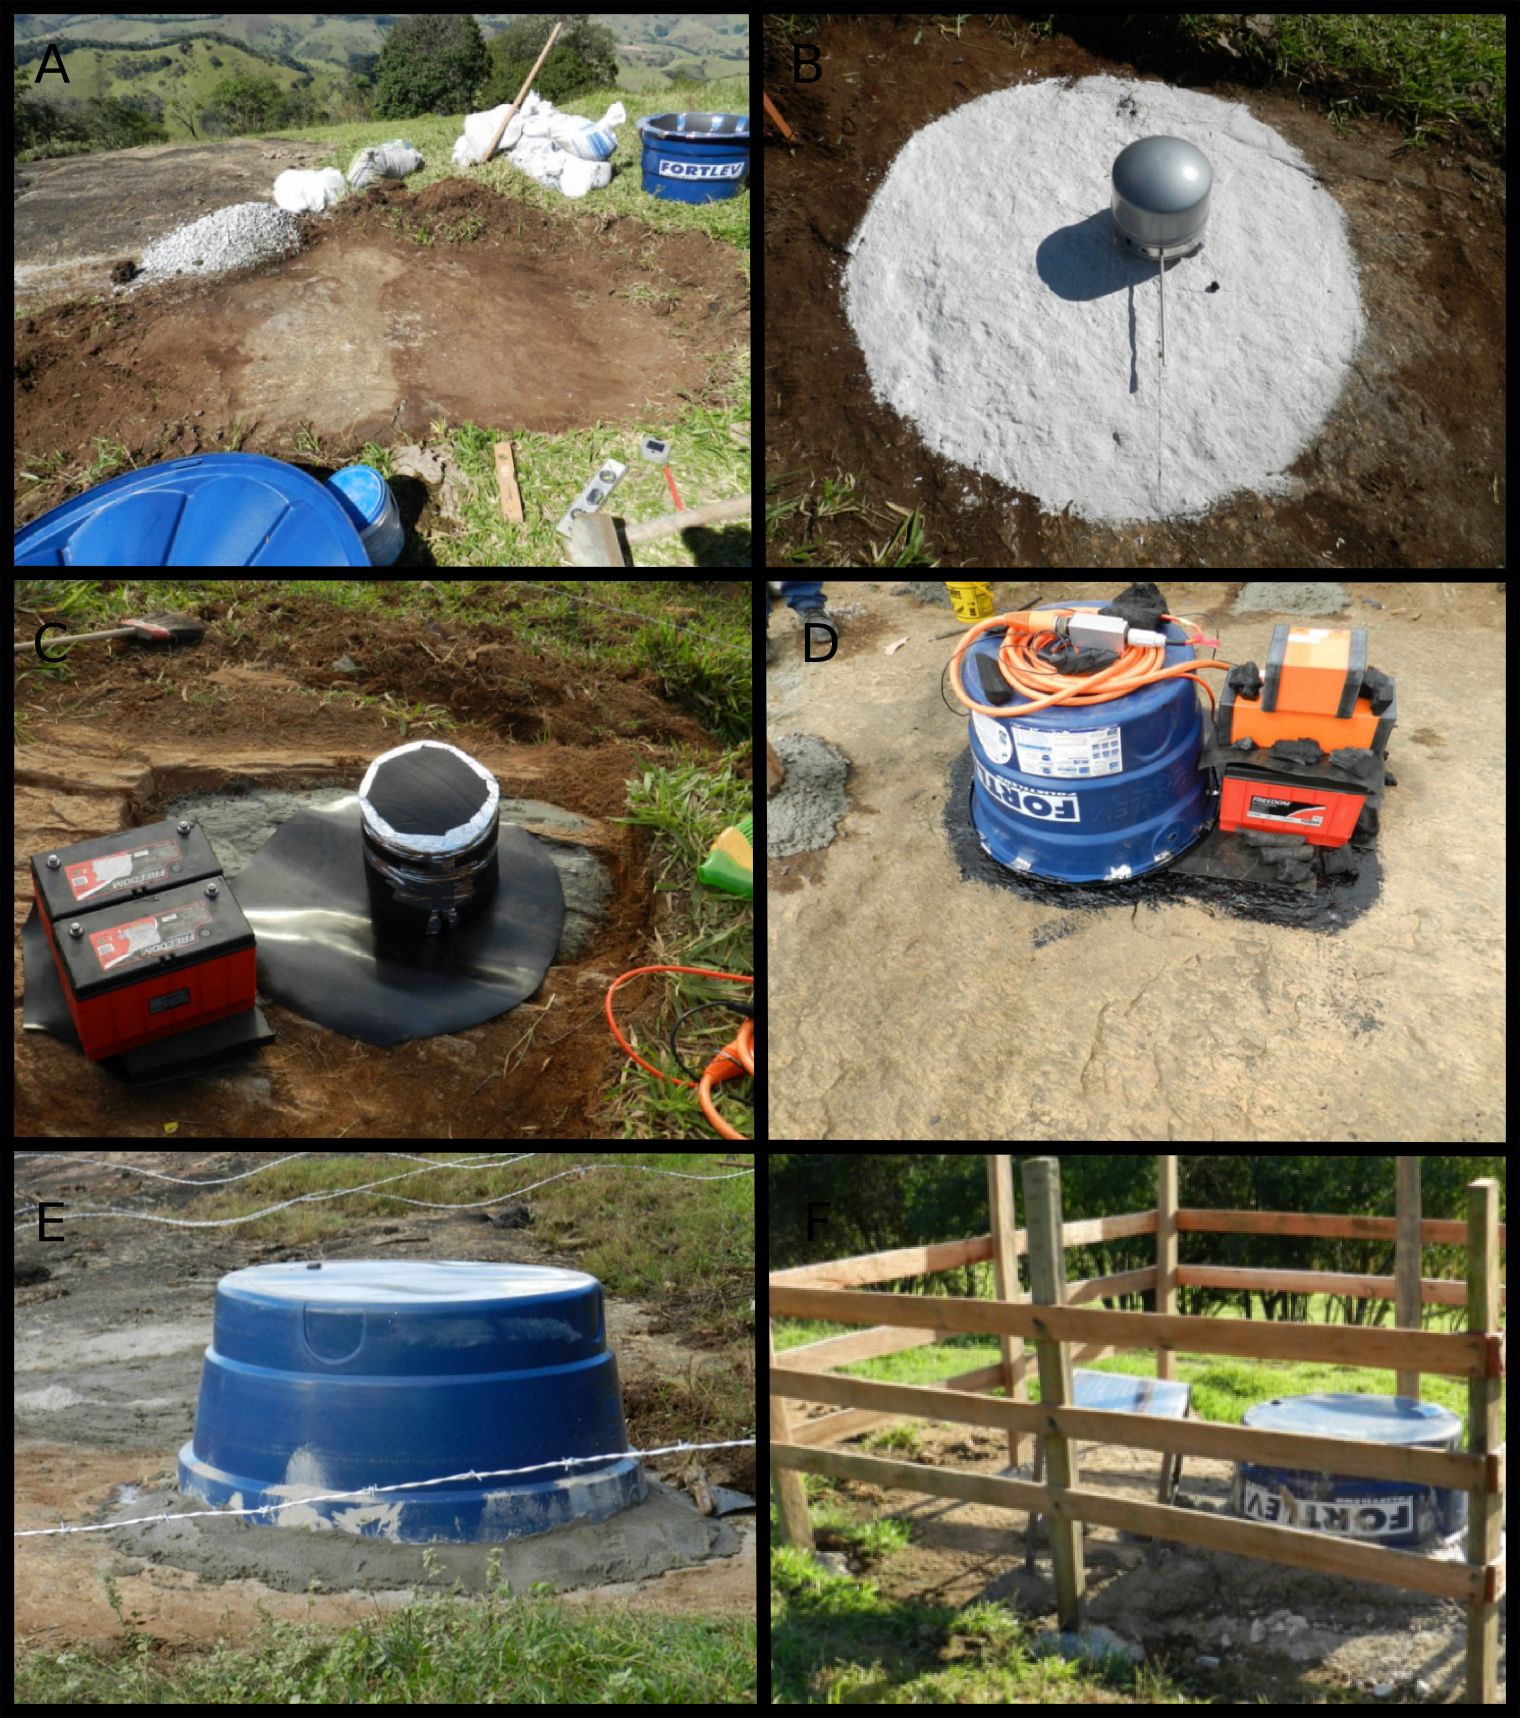
\includegraphics[scale=0.5]{Figs/instalacao.png}
\caption[Mosaico mostrando como é feita a instalação das estações sismográficas temporárias do projeto SUBSAL.]{Mosaico mostrando como é feita a instalação das estações sismográficas temporárias do projeto SUBSAL. As figuras mostram os diferentes estágios na instalação das estações.}
\label{instalacao}
\end{figure} 

As estações foram dispostas espacialmente em três perfis em relação à costa, dois perpendiculares à costa, perfil 1 a oeste e perfil 2 a leste, e um paralelo, perfil 3, como observado na Figura \ref{map_loc}. A distância entre as estações é aproximativamente de 20 km. As coordenadas das estações estão listadas na Tabela \ref{tabelaDATA}. 

\begin{figure}[!ht]
\centering
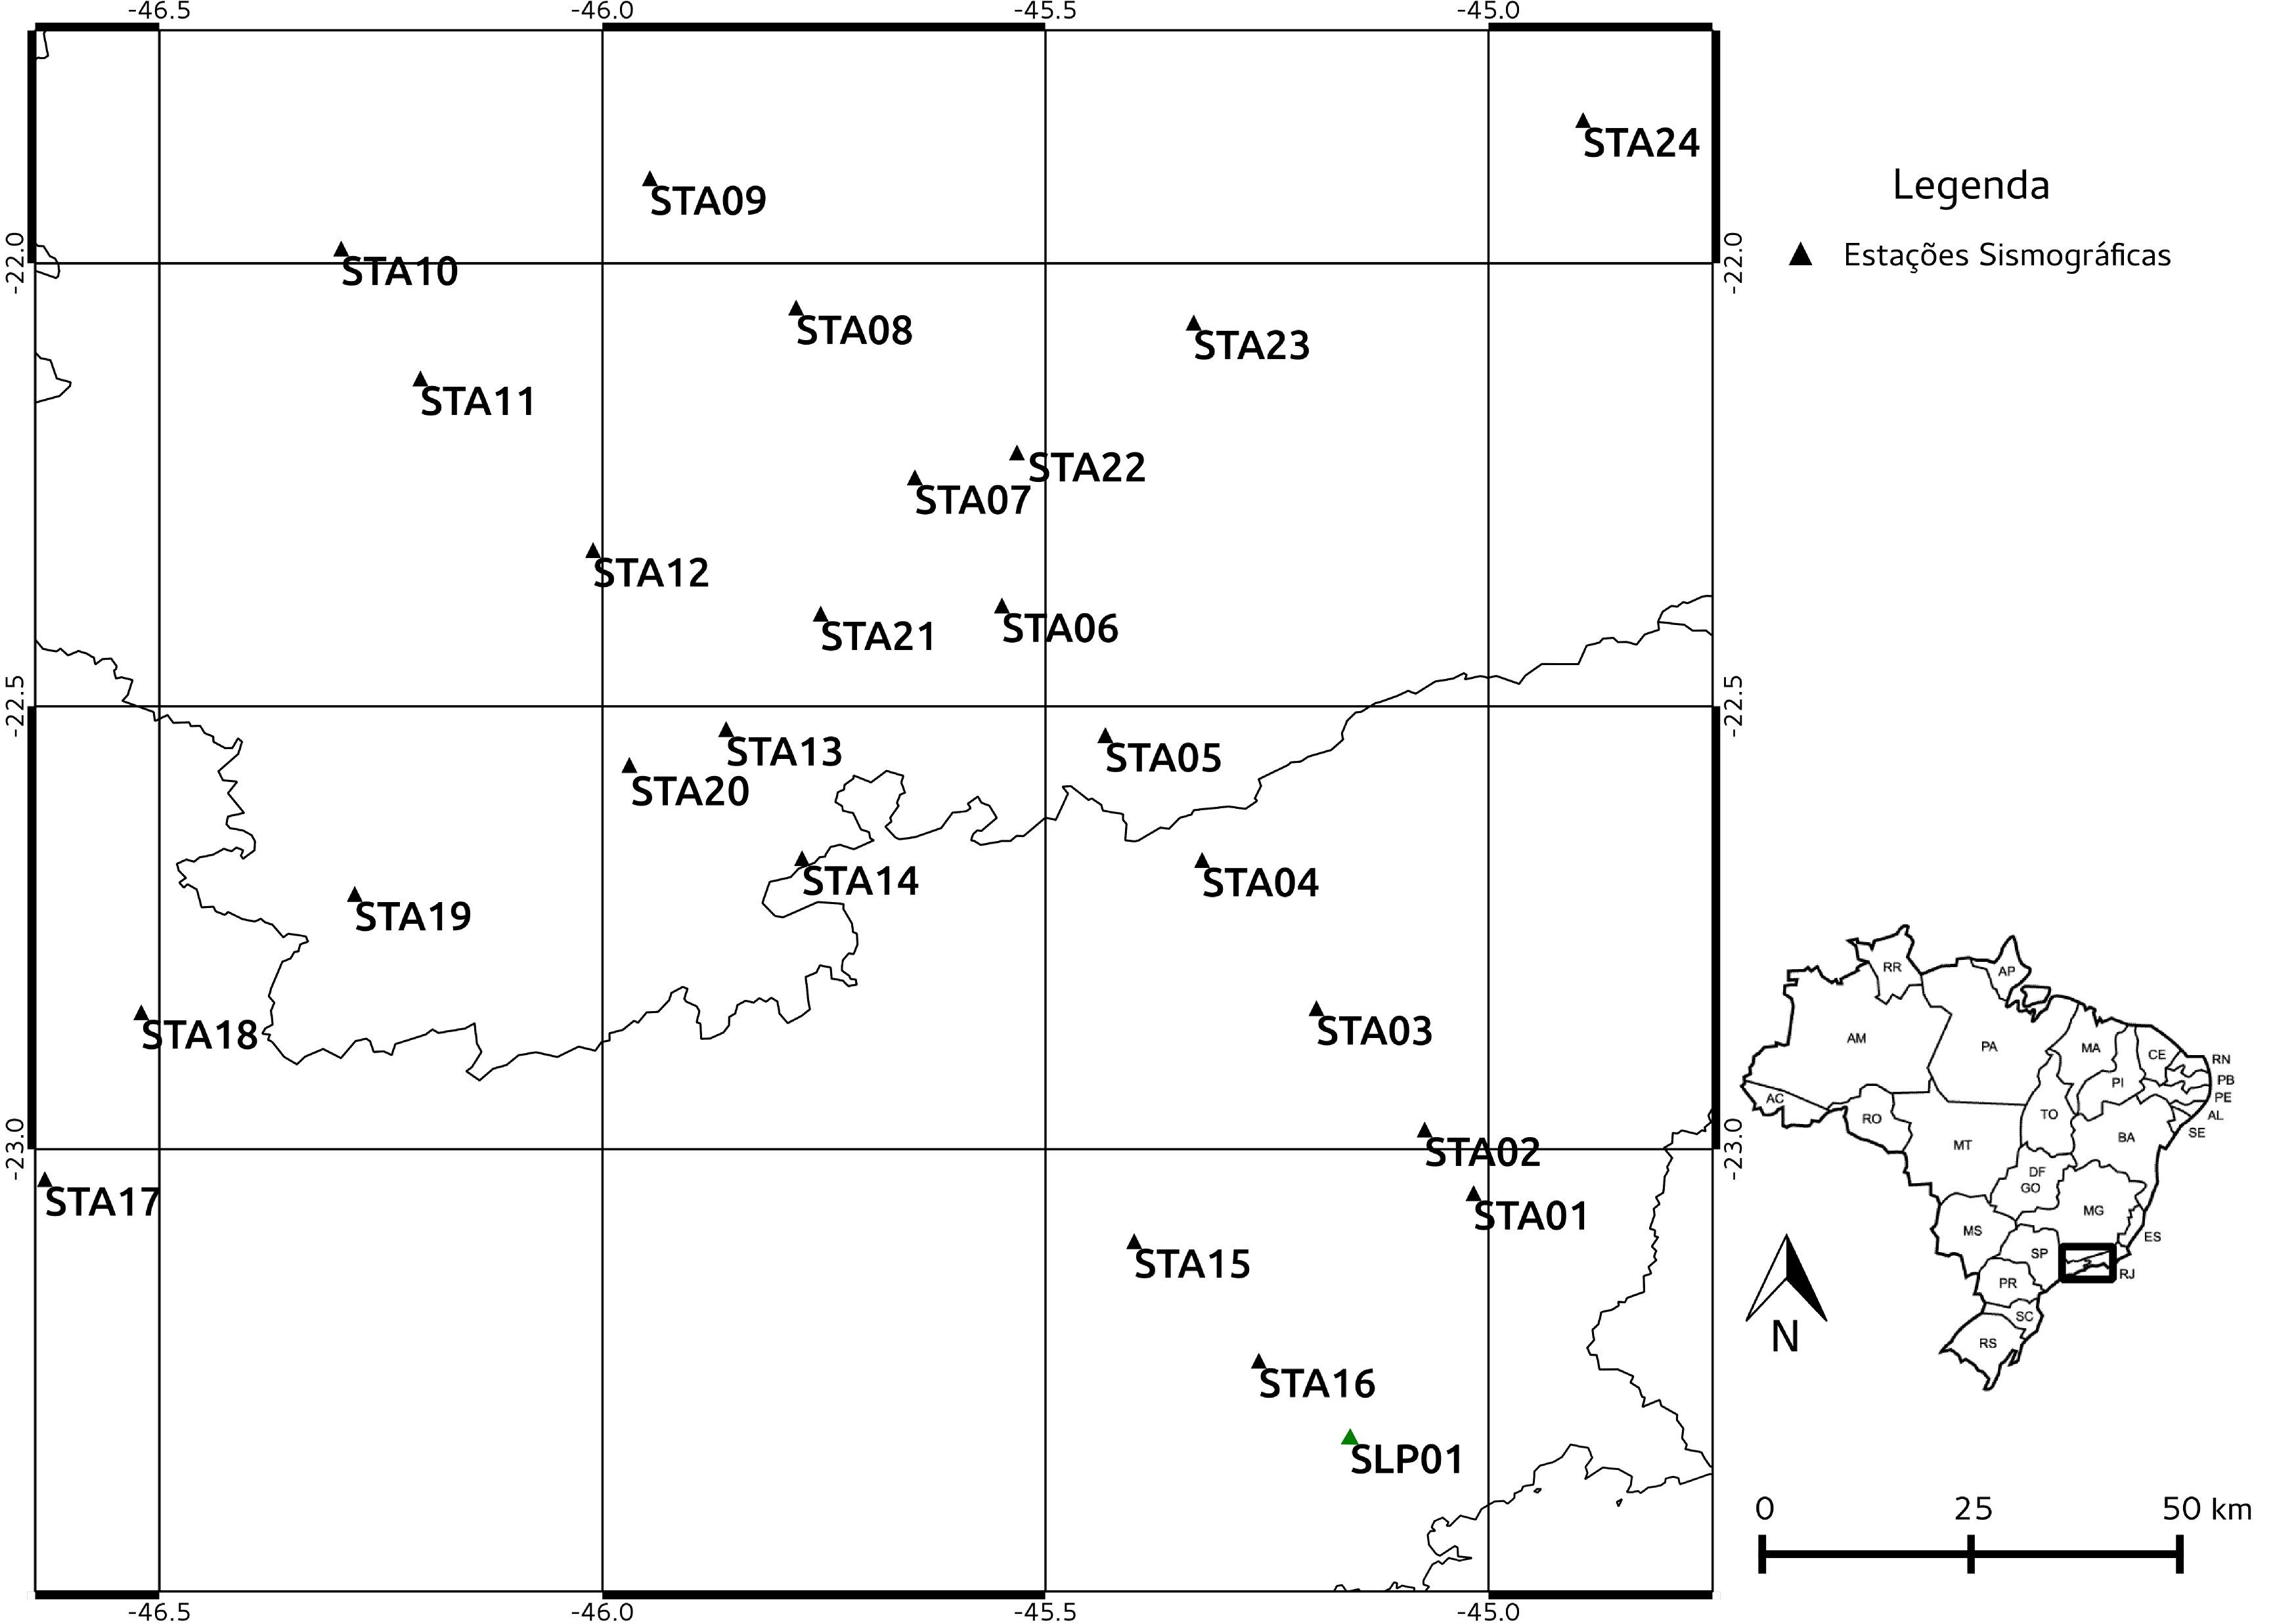
\includegraphics[scale=0.5]{Figs/mapa_das_estacoes_simosgraficas_instaladas.png}
\caption{Mapa das estações sismográficas instaladas (triângulos vermelhos). Os outros triângulos são estações da Rede Sismográfica Brasileira. O perfil 1 estende-se da estação STA01, localizada próximo à costa, até a STA09. O perfil 2 vai da estação STA10, ao norte, até a STA16, próximo à costa. Já o perfil 3 é da estação STA17, oeste, até a STA24, leste.}
\label{map_loc}
\end{figure}

O período de operação das estações foi distinto para os perfis. Os dois perfis perpendiculares à costa foram instalados no meio do ano de 2012 e o perfil paralelo no final de 2012. As estações ficaram em fucionamento até o final do ano de 2013 registrando o movimento do terreno, as datas em que as estações ficaram em funcionamento podem ser encontradas na Tabela \ref{tabelaDATA}. 

A velocidade do meio é registrada pelo sismógrafo, dado bruto, através de sensores verticais e horizontais. Pode ser visto na Figura \ref{simograma} o deslocamento do meio que é encontrado através da integração matemática dos registros de velocidade. Esse registro da variação da amplitude resultante da integração em uma série temporal é chamado de sismograma. 

\begin{figure}[!ht]
\centering
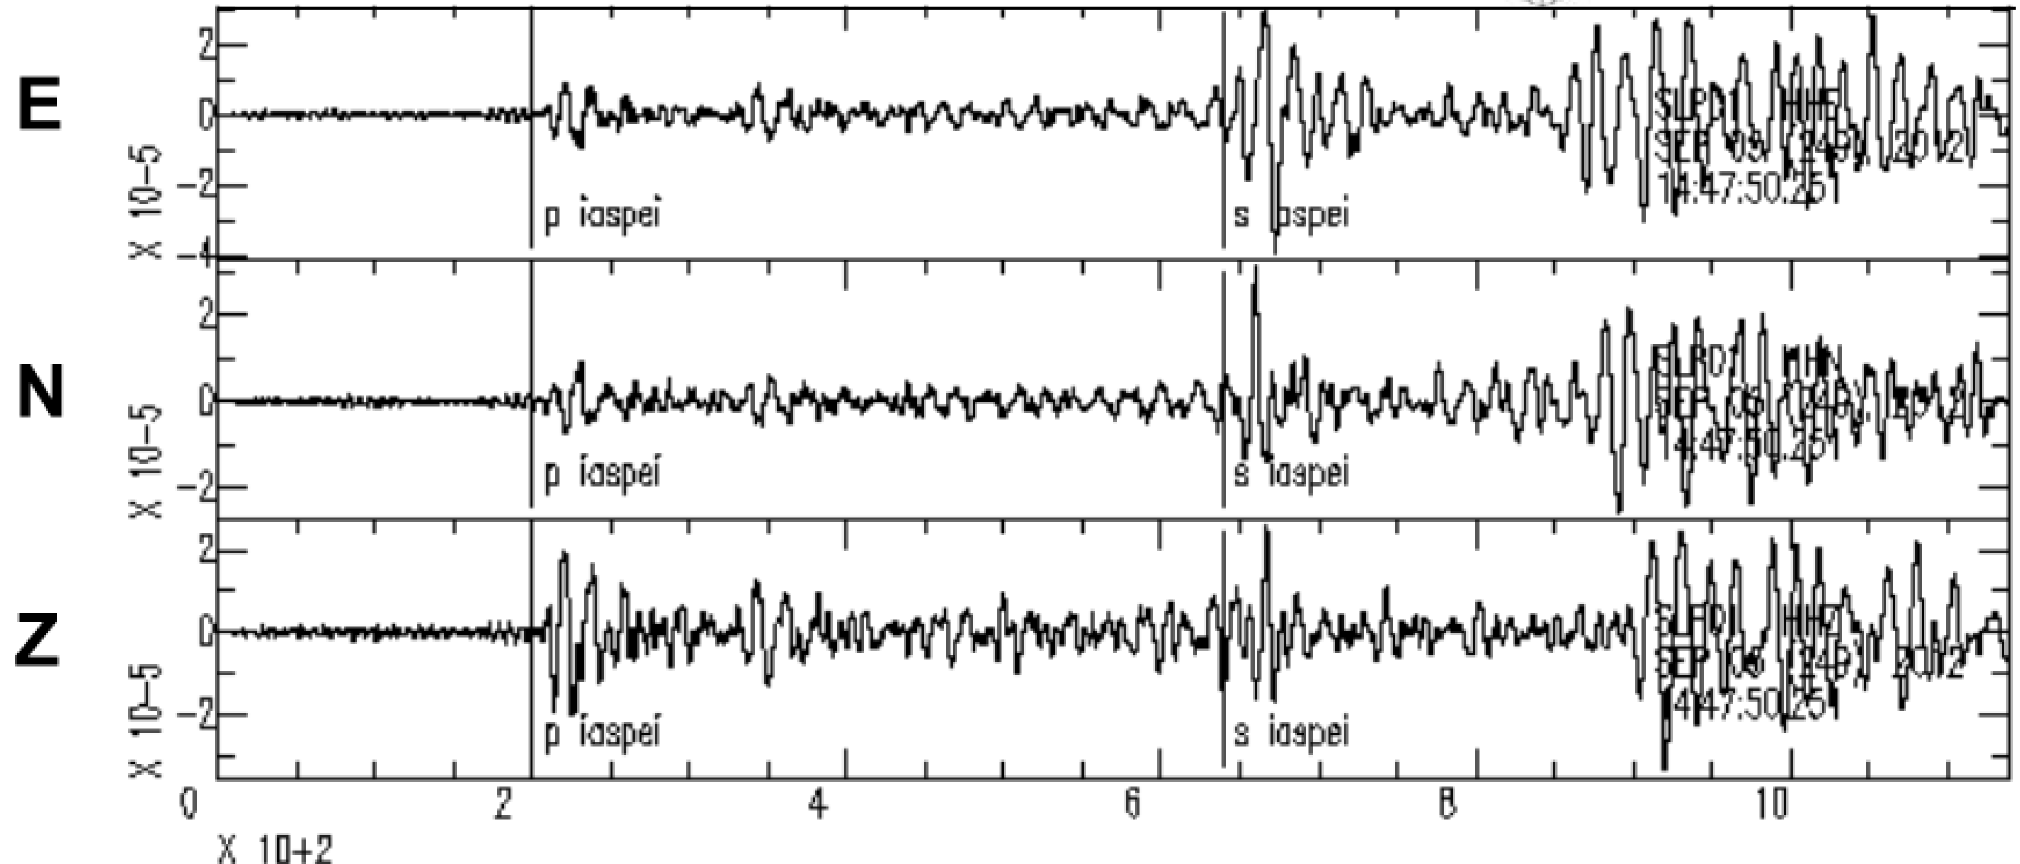
\includegraphics[scale=0.6]{Figs/sismograma.png}
\caption{Sismograma mostrandos as três componentes do deslocamento do terreno.}
\label{simograma}
\end{figure}

O sismograma é gerado pela perturbação do meio pelas ondas  mecânicas que se propagam no interior da Terra. As velocidades ondas variam em função dos parâmetros elásticos do meio e da densidade, estes variam pela mineralogia e condições de pressão e temperatura do meio atravessado. As ondas mecânicas são divididas em ondas de corpo e de superfície. As ondas de corpo estão categorizadas em dois tipos: as ondas P, longitudinais, e as ondas S, transversais. A onda P é mais rapida e consegue se propagar em todos os meios, tem velocidade entre 4 e 7 km$/$s na crosta terrestre e em torno de 8 km$/$s no manto superior. As ondas S tem velocidade menor, em torno de 3 a 4 $km/$s na crosta, porém a onda S não se propaga em meios líquidos.

Para produzir esta análise sobre a estrutura da região de estudo pelo método da Função do Receptor, \cite{langston_structure_1979},utilizou-se de um conjunto de dados com eventos sísmicos registrados. Já para a Dispersão de Ondas de Rayleigh, \cite{campillo_long-range_2003} e \cite{shapiro_emergence_2004}, utilizou-se o ruído sísmico ambiental.

\section{Tratamento dos Dados}

A caracterização prévia das informações contidas no sinal é imprescindível para o processamento. A primeira avaliação da performance e da qualidade dos dados da estações sismográficas foram feitas no software livre PQLX.  A metodologia do PQLX é baseada no trabalho de \cite{McNamara_Buland_2004}. Esse procedimento é bastante usado para se obter a informação espectral sísmica.

A metodoliga de \cite{McNamara_Buland_2004} segmenta a série temporal em intervalos de uma hora, com 50\% de superposição do sinal. Cada janela de hora está separada em 13 intervalos com 75\% de superposição para calcular a densidade de potência espectral, \textit{Power Spectral Density}. As médias obtidas para cada um dos 13 intervalos são usadas para estimar as funções densidade de probabilidade, \textit{Probability Density Functions}, calculados a partir das médias pelo número total de segmentos de hora em hora. 

Essa metodologia de \cite{McNamara_Buland_2004} difere dos métodos habitualmente utilizados, porque não é necessário a visualização de todo conjunto de dados para uma estima qualitativa do sinal.

\begin{figure}[!ht]
\centering
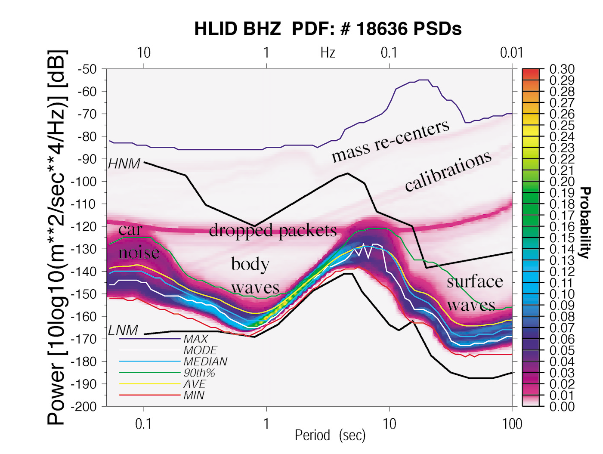
\includegraphics[scale=0.6]{Figs/mcnamura_buland.png}
\caption[Análise qualitativa do sinal atraves das funções densidade de probabilidade]{Análise qualitativa do sinal atraves das funções densidade de probabilidade,\textit{Power Density Functions}, segundo \cite{McNamara_Buland_2004}. As curvas HNM e LNM, que são o maior nível de ruído  e o menor nível de ruído, respectivamente. Estes são valores padrões de diferentes estações, são utilizados para demarcar o limite mínimo e máximo que o nível de ruído pode chegar. A funções densidade de probalibilidade mostram a distribuição das fontes de ruído sísmico. Altas frequências são dominadas por ondas de volume e períodos longos por ondas de superfícies. Como por exemplo, ruído antrópicos de alta frequência. Ruídos gerados por vento, água e pelo contexto geológico local se apresentam em períodos mais longos. Microssismos apresentam dois picos bem marcantes no espectro do ruído sísmico ambiental, um de 10-16 segundos conhecido como "pico de frequência único. Em altas amplitudes, picos de longo período, de 4-8 segundos encontram-se os "picos de frequênacia dupla".}
\label{PQLX}
\end{figure}

O produto de uma análise qualitativa preliminar nos gráficos gerados pelo programa PQLX é mostrado na Figura \ref{PQLX_results}, que tem como exemplos a componente HHZ nas estações STA05, STA04 e STA24. Observando os resultados nas estações temporárias conclui-se que existem registros bons e confiáveis, como exemplo a Figura \ref{PQLX_results}-A. Porém em algumas estações existem pequenos problemas, que são caracterizados por tendências lineares, como observados na Figura \ref{PQLX_results}-B. Já em outras estações pode-se constatar a falta de registros na componente HHZ,   possíveis problemas instrumentais, observado na Figura \ref{PQLX_results}-C.

\begin{figure}[!ht]
\centering
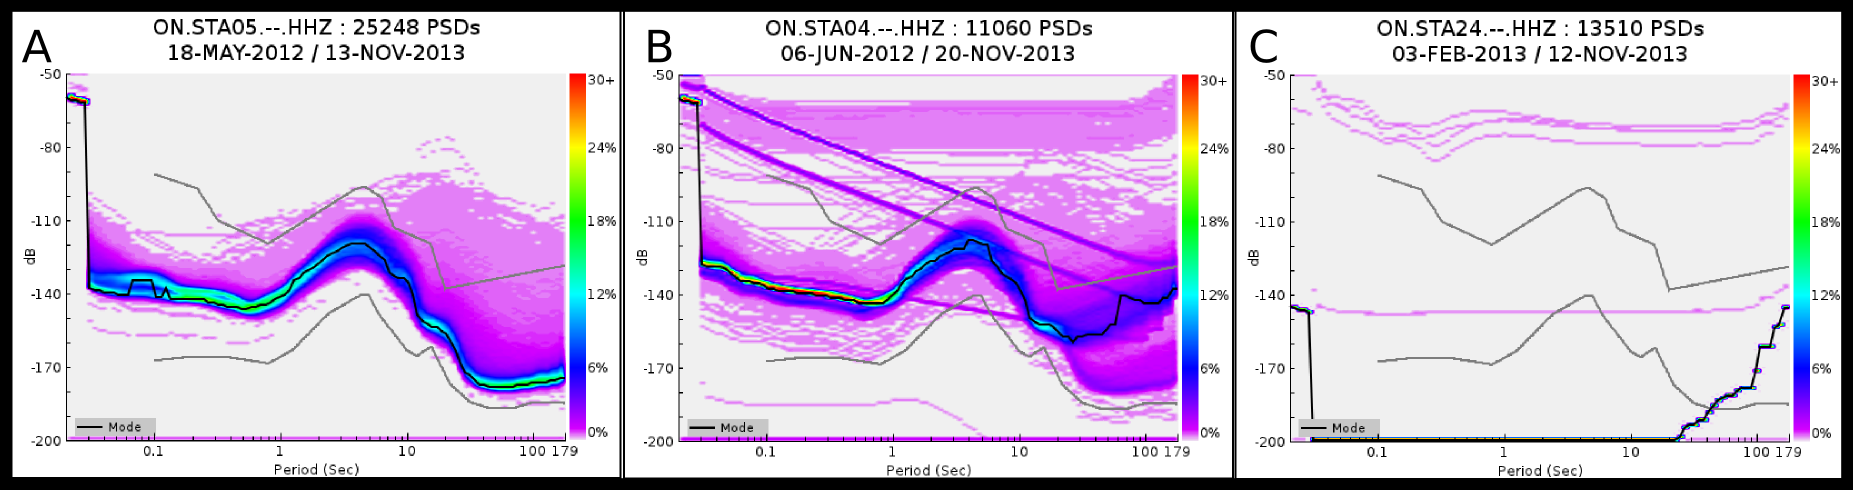
\includegraphics[scale=0.35]{Figs/pqlx_results.png}
\caption{Exemplos de resultados gerados pela análise qualitativa do sinal atraves do programa PQLX, que utiliza o método de \cite{McNamara_Buland_2004}.}
\label{PQLX_results}
\end{figure}

\subsection{Processamento da Função do Receptor}

Os dados utilizados para os cálculos da Função do Receptor foram dados coletados em 24 estações temporárias da Rede SUBSAL e na estação permanente SLP01, esta pertencente a rede RSIS, parte da Rede Simosgráfica Brasileira (RSB), \url{www.rsbr.gov.br}, observado na Figura \ref{map_loc}. Porém ao final agregou-se estações pertencentes à Universidade de São Paulo (USP), citados por \cite{Assumpcao_Brazil_2013}. 

Para assegurar a confiabilidade do processamento é necessário um tratamento preliminar dos sinais. Utilizou-se eventos catalogados na rede IRIS,\textit{Incorporated Research Institutions for Seismology}\url{http://www.iris.edu/hq/}, para uma identificação automática nestes sinais. Alguns pré-requisitos foram utilizados para a escolha dos eventos, como:

\begin{enumerate}
\item Distância Epicentral (Entre 20º e 95º);
\item Magnitude;
\end{enumerate}

A distância epicentral é tida como ideal entre 20 e 95 graus, como é observado na Figura \ref{mapa_eventos}. Sismos próximos (distância menor que 20 graus) geram ondas com incidência oblíqua e produzem uma triplicação característica. Esta se refere a fases de ondas sísmicas que possuem um parâmetro do raio similar e possuem os tempos de chegada das reflexões das ondes bem próximos, \cite{stahler_triplicated_2012}, logo devem ser processados de maneira diferente. Em sismos com distâncias maiores que 95 graus as ondas P não chegam na estação devido a inversão de velocidade no limite manto-núcleo, diminuição da velocidade da onda P entre o manto e o núcleo, e não é observada a onda P direta. Devido grande parte dos sismos serem oriundos da Cordilheira dos Andes,como é visto na Figura \ref{teste_tempo}, também utilizou-se dados com distâncias menores que 20 graus. A magnitude do sismo é importante para a propagação da onda, eventos com pequena magnitude não tem energia suficiente para gerar um sinal claro no sismograma.

\begin{figure}[!ht]
\centering
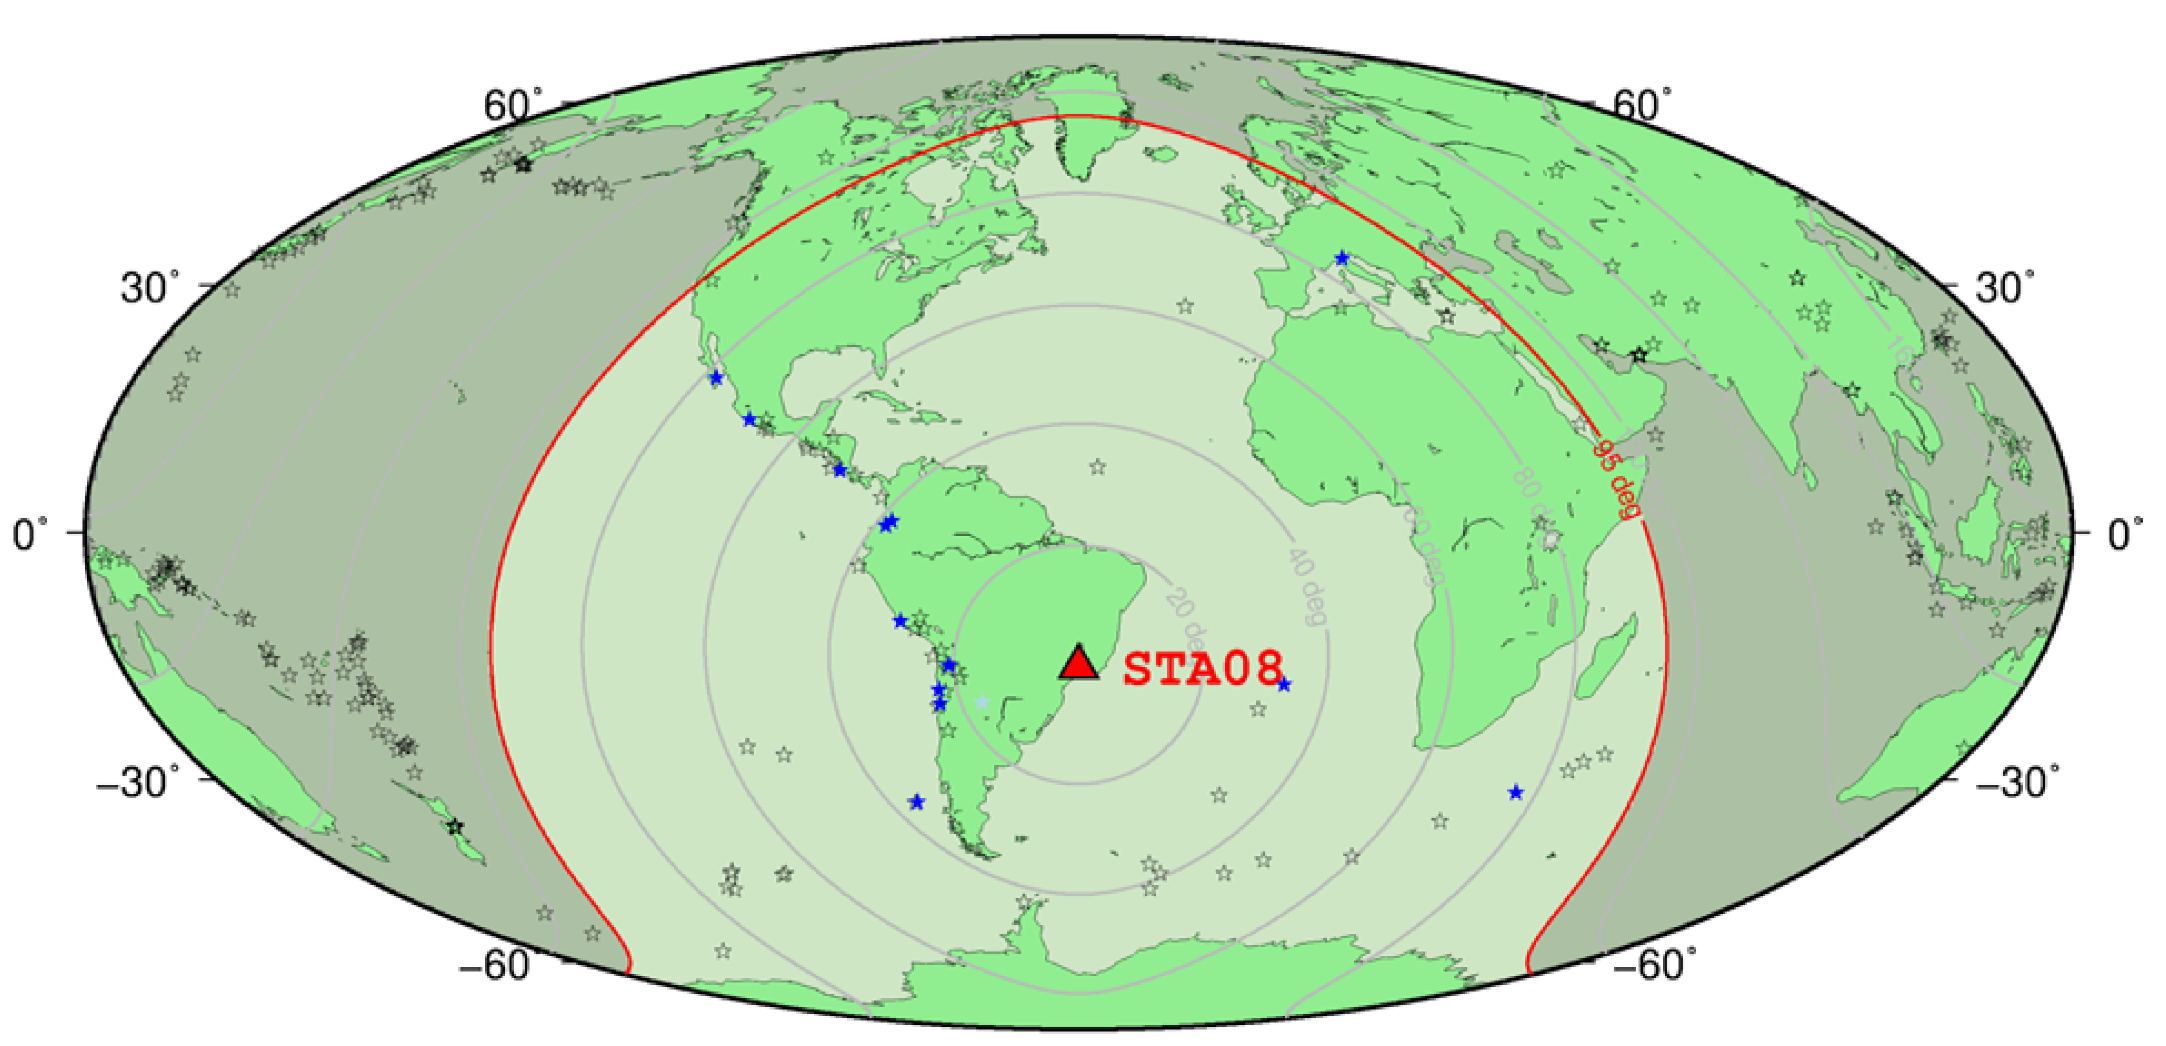
\includegraphics[scale=0.6]{Figs/mapa_de_eventos.png}
\caption[Mapa dos eventos registrados na estação STA08.]{Mapa dos eventos (estrelas) registrados na estação STA08. O limite de 95 graus está indicada em vermelho. Estrelas azuls mostram os eventos com dados de qualidade que são usadas no calculo das Funçoes do Receptor}
\label{mapa_eventos}
\end{figure}

Para análise 

Subsequentemente foi feito um janelamento no dado do evento 5 segundos antes e 10 segundos depois da chegada da onda P, como visto na Figura \ref{simograma}. Após a discriminação e o janelamento do sinal, examina-se visualmente cada registro para certificar que todos os eventos selecionados tem um nível de sinal-ruído bom e fazer a marcação do tempo de chegada da onda P, como na Figura \ref{simograma}. No sinal observado é marcado o tempo de chegada da onda P. O tempo de chegada da onda P é calculada pelo modelo de velocidade da Terra IASPEI91 de \cite{kennet_iaspei_1991}.

Logo após removeu-se a média e tendência linear dos dados. Aplicou-se um filtro passa-alta com freqüência de corte de 0.1 Hz para eventos com distância entre 20 e 95 graus e de 2 Hz para eventos próximos ($<$20). Os dados originais são reamostrados e interpolados de 0,01 segundos (100 Hz) para 0,025 segundas (40 Hz), porque a informação de alta freqüência não é considerada nesta análise.

Após esta análise preliminar observou-se que algumas estações temporárias, STA22, STA23 e STA24, apresentaram problemas e foram descartadas dessa análise. As estações STA23 e STA24 apresentaram a componente vertical quebrada, porém as outras componentes estão aptas e serem utilizadas em outros estudos, como Dispersão das Ondas Love. Já a estação STA22 foi descartada pelo curto período de funcionamento, como pode ser visto na Tabela \ref{tabelaDATA}.


\subsection{Dispersão de Ondas de Rayleigh}

Para o cálculo da dispersão das ondas de superfície utilizou-se estações temporárias da Rede SUBSAL, estações da Rede GEOSCOPE, pertencentes ao \textit{Institut de Physique du Globe de Paris} e do Projeto de Sísmica  da Litosfera Brasileira, pertencentes a Universidade de São Paulo (USP).

A garantia da fiabilidade do tempo de chegada da onda P é fundamental para o processamento gerar resultados consistentes. Pois, ao contrário do método da Função do Receptor que usa registros de uma mesma estação, o método da Dispersão de Ondas de Superfície utiliza dados de duas estações, logo tais estações devem estar sincronizadas. \cite{gibbons_identification_2006} mostra que ao fazer a correlação cruzada de dois eventos distantes em uma estação sismográfica consegue-se caracterizar esse tempo de chegada, como é visto na Figura \ref{teste_tempo}. Ele assume que se não há alterações mensuráveis na velocidade da estrutura entre a fonte e os receptores, as ondas sísmicas de dois eventos co-localizados terão a mesma duração de tempo para chegar a um determinado sensor. Qualquer discrepância nos tempos de separação medido em duas estações diferentes, o que não é atribuível a diferença entre fontes ou uma SNR baixa, deve ser o resultado de uma anomalia em sincronismo um, ou ambos, dos instrumentos.

\begin{figure}[!ht]
\centering
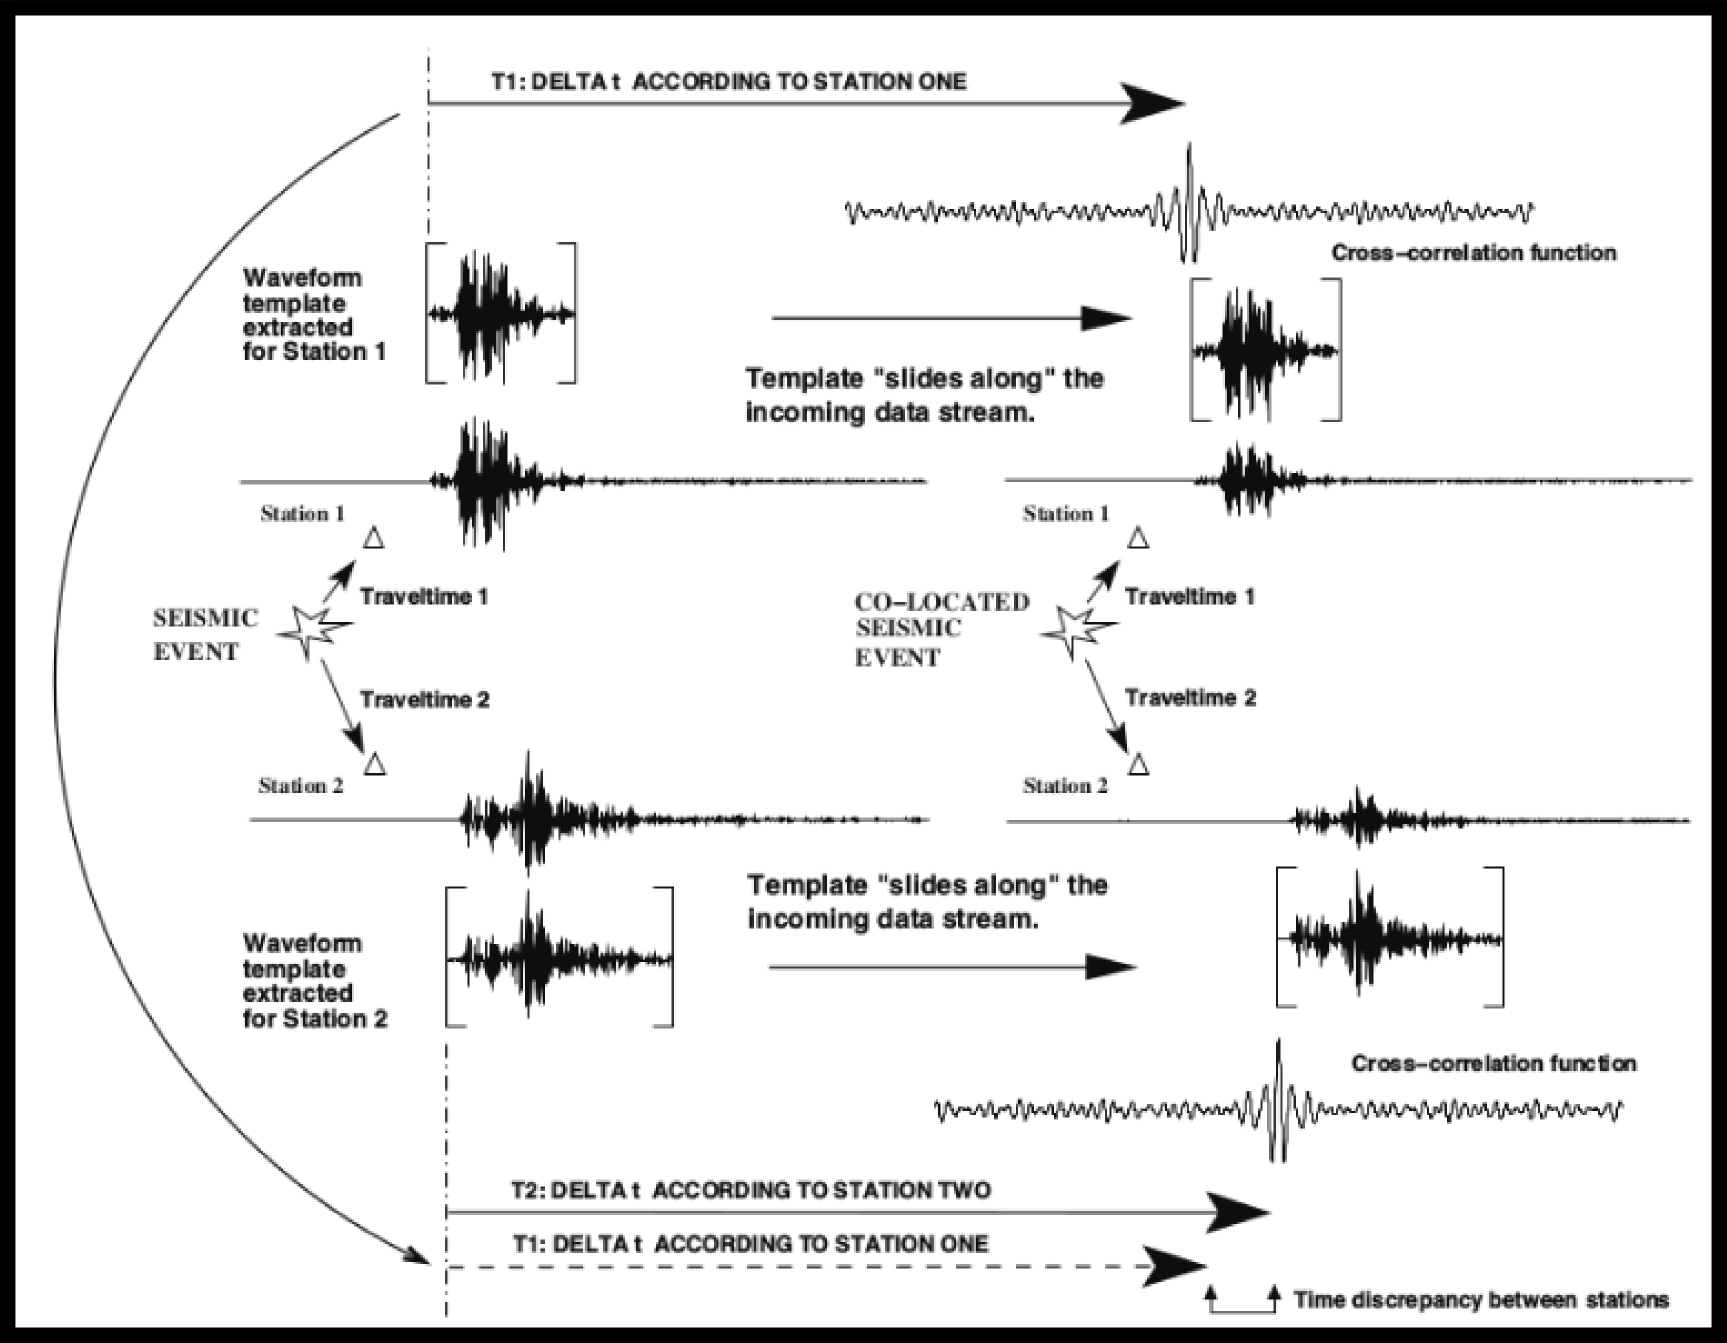
\includegraphics[scale=0.7]{Figs/correlacao_tempo_de_chegada.png}
\caption[Uma ilustração esquemática mostrando a correlação dos tempos de chegada da onda P.]{Uma ilustração esquemática de como dois eventos sucessivos de fontes sísmicas quase idênticas que podem ser explorados para revelar anomalias dos tempo de chegada da onda P numa dada estação. \cite{gibbons_identification_2006}}
\label{teste_tempo}
\end{figure}

Neste trabalho utilizamos uma metodologia conceitualmente semelhante a de \cite{gibbons_identification_2006}. Fez-se a correlação cruzada dos dados de um sismo distante de um par de estações sismográficas próximas. Como a fonte está distante das estaçõesm, a correlação cruzada dos sinais deve ser próxima de zero. A estação SLP01 foi utilizada como referência devido a proximidade com as estações do rede SUBSAL. 

\begin{figure}[!ht]
\centering
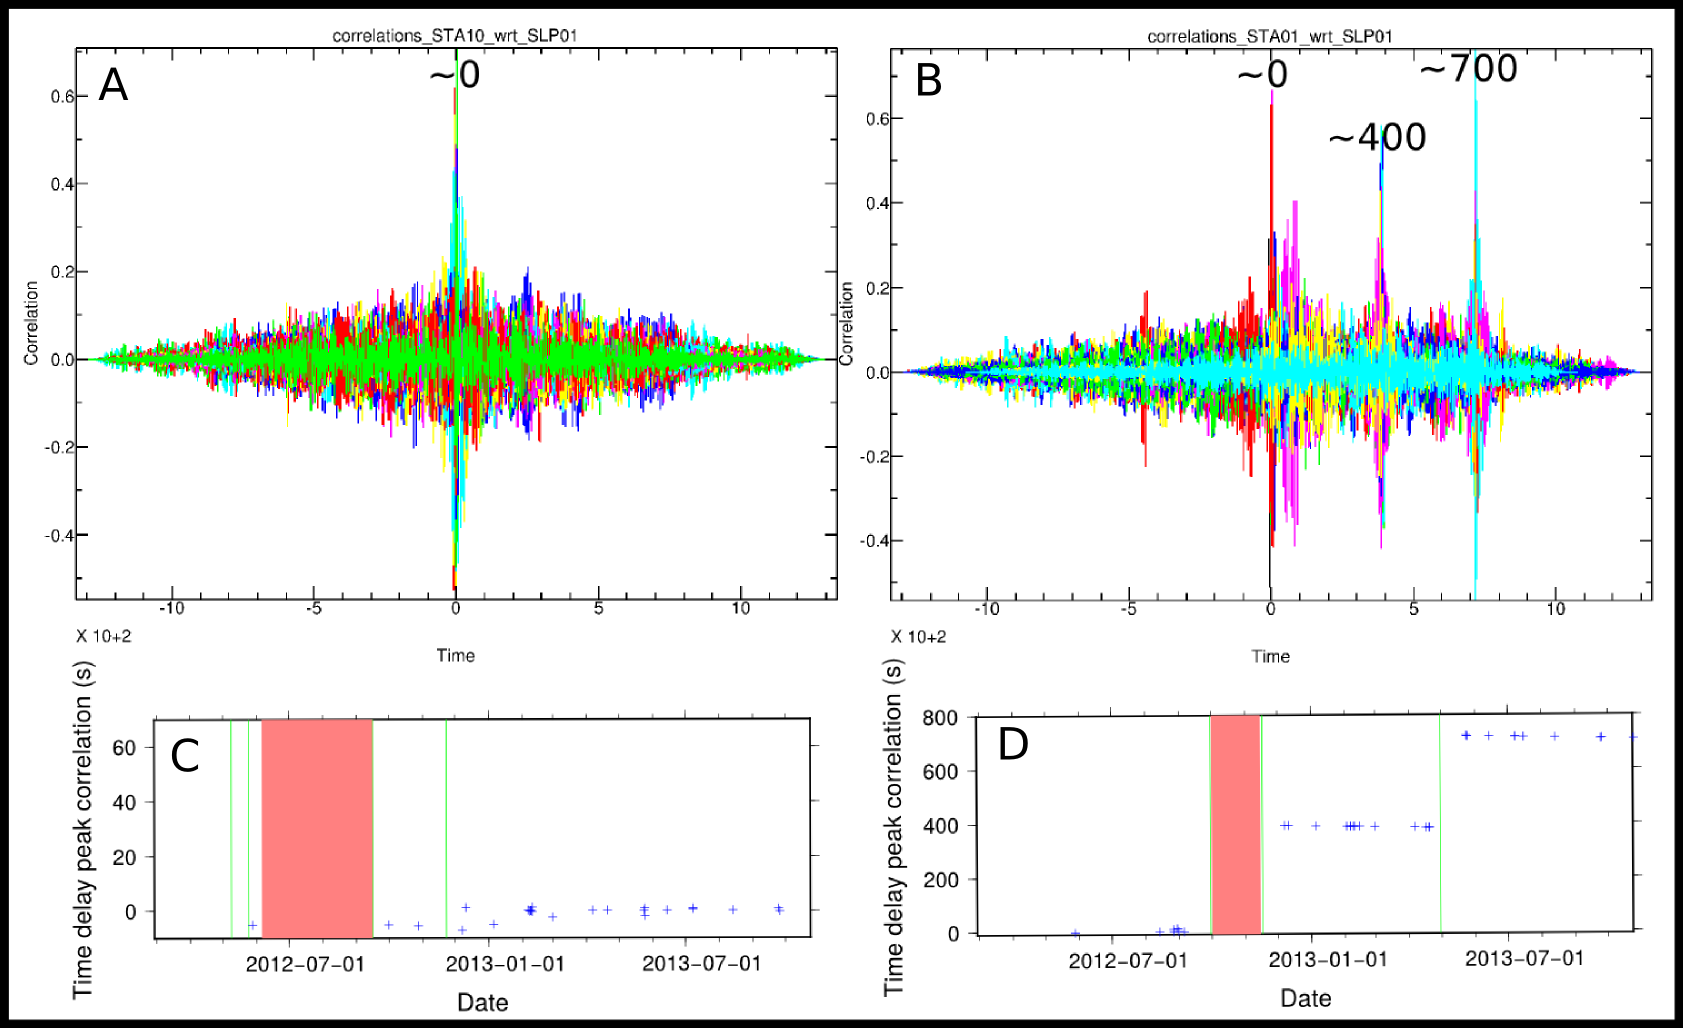
\includegraphics[scale=0.3]{Figs/correlacao_tempo_de_chegada_resultado.png}
\caption[Correlação de eventos sucessivos de fontes sísmicas entre duas estações sismográficas]{Correlação de eventos sucessivos de fontes sísmicas entre as estações sismográficas STA10 e SLP01 (A) e  STA01 e SLP01 (B). Na parte inferior mostram o atraso do tempo de chegada da onda P da correlação pelo tempo. As retas verticais verdes mostram os períodos onde teve manutenção do equipamento e as em vermelhas quando a estação não estava funcionando (C e D).}
\label{teste_tempo_results}
\end{figure}

Os gráficos gerados com a correlação cruzada são vistos na Figura \ref{teste_tempo_results}. Os resultados mostram que para algumas estações temporárias há uma defasagem no tempo de chegada da onda P, Figura \ref{teste_tempo_results}-B. Tais defasagens podem ter sidos gerados por difentes fatores, como erro no sinal do GPS acoplado à estação, erro instrumental. As Figuras \ref{teste_tempo_results}-C e \ref{teste_tempo_results}-D apresentam a defasagem das correlações cruzadas. Nota-se uma relação entre os  dias que ocorreram manutenções nas estações  e a ocorrência de defasagem no sinal, essas manutenções estão demarcados pelas linhas verticais verdes na Figuras \ref{teste_tempo_results}-C e \ref{teste_tempo_results}-D. A Figuras \ref{teste_tempo_results}-D mostra que a estação STA01 apresenta um aumento sistemático na defasagem medida, estes números, 400 e 700 segundos, são verificados na Figura \ref{teste_tempo_results}-B.

Com esse tratamento preliminar dos dados pôde-se selecionar melhor o banco de dados, com isso  e tentar minimizar os erros gerados no processamento da dispersão das curvas de superfície. Após estes estudos, as estações temporárias STA23 e STA24 foram consideradas impróprias para o cálculos da dispersão das ondas Rayleigh. Porém serão aproveitadas quando for analisada a dispersão das ondas Love, pois as componentes horizontais estão boas. A estação STA22 só possui 4 dias de dados registrados, logo foi descartada da análise.
